\documentclass[tikz]{standalone}
\usepackage{tikz}
\usetikzlibrary{automata, positioning}

\begin{document}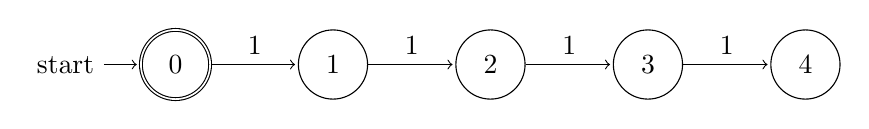
\begin{tikzpicture}[shorten >=1pt, node distance=2cm, on grid, auto]

  % Nodes in a horizontal line
  \node[state, initial, accepting] (q0) {0};
  \node[state, right of=q0] (q1) {1};
  \node[state, right of=q1] (q2) {2};
  \node[state, right of=q2] (q3) {3};
  \node[state, right of=q3] (q4) {4};

  % "inc" transitions from 0 to 9
  \path[->] (q0) edge node {1} (q1);
  \path[->] (q1) edge node {1} (q2);
  \path[->] (q2) edge node {1} (q3);
  \path[->] (q3) edge node {1} (q4);

\end{tikzpicture}
\end{document}
